% --------------------------------------------------------------
% This is all preamble stuff that you don't have to worry about.
% Head down to where it says "Start here"
% --------------------------------------------------------------
 

\pdfminorversion=7 
% \PassOptionsToPackage{dvipdfmx}{graphicx}
\documentclass{beamer}
\usepackage[english]{babel} 
\usepackage[utf8]{inputenc} 
\usepackage{graphicx}
\usetheme{Madrid}
\usecolortheme{whale}

%------------------------------------------------------------
%This block of code defines the information to appear in the
%Title page
\title[AI and ML] %optional
{Intro to AI and ML}
\subtitle{MATRIX PROJECT}
\author[Anjani Kumar, Tungadri Mandal] % (optional)
{Anjani Kumar : CS17BTECH11002\inst{1} \\ \and Tungadri Mandal : CS17BTECH11043\inst{2}}

\institute[] % (optional)
{
  \inst{1, 2}
  Indian Institute of Technology, Hyderabad\\

}


%End of title page configuration block
%------------------------------------------------------------

%------------------------------------------------------------
%The next block of commands puts the table of contents at the 
%beginning of each section and highlights the current section:

\AtBeginSection[]
{
  \begin{frame}
    \frametitle{Table of Contents}
    \tableofcontents[currentsection]
  \end{frame}
}
%------------------------------------------------------------

\begin{document}
 
% --------------------------------------------------------------
%                         Start here
% --------------------------------------------------------------

\frame{\titlepage}

% Frame 2
\begin{frame}
\frametitle{Problem Statement }
Original Question\\
Find the equation of the circle which is the mirror image of the circle\\
\begin{equation}
    \boldsymbol{{x^2}+{y^2}-2x=0}
\end{equation}
about the line\\
\begin{equation}
    \boldsymbol{y=3-x}
\end{equation}
\end{frame}
%% Frame 2 end

% Frame 3
\begin{frame}
\frametitle{Problem Statement }
Matrix Form\\
Find the equation of the circle, which is the
mirror image of the circle
\begin{equation}
    \boldsymbol{x^Tx} - (2\hspace{5mm} 0)\boldsymbol{x} = 0
\end{equation}
in the line 
\begin{equation}
    (1\hspace{5mm} 1)\boldsymbol{x} = 3
\end{equation}
\end{frame}
% Frame 3 end

% Frame 4
\section{Desired Answer}
\begin{frame}{Desired Answer}
% An image of the given circle, line and it's mirror image attached
\begin{figure}[h]
\centering
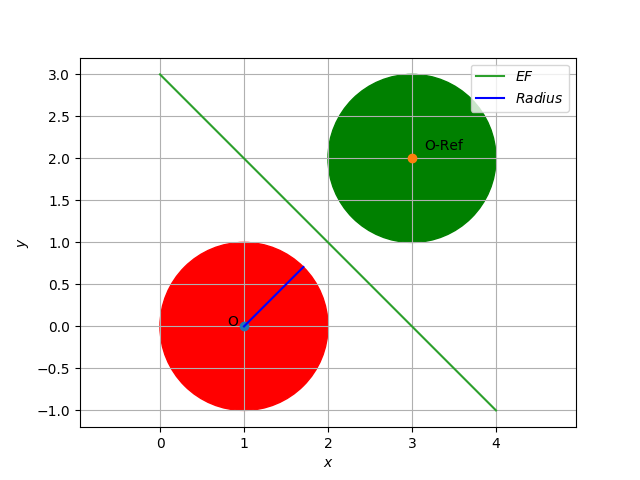
\includegraphics[scale=0.54]{figs/circles.png}
\caption{Reflection of circle about a line}
\label{etiqueta}
\end{figure}
\end{frame}
%Frame 4 end

% Frame 7
\section{Approach1}
\begin{frame}{Using foot of the $\bot$ from center to the line}
\begin{solution}
Let $\boldsymbol{c}$ be the center and r be the radius of the circle respectively.
\begin{equation}
    \Vert\left(\boldsymbol{x - c}) \right\Vert^2 = r^2
\end{equation}
\begin{equation}
    \Rightarrow \boldsymbol{(x-c)^T(x-c)} = r^2
\end{equation}
\begin{equation}
    \Rightarrow \boldsymbol{x^Tx - 2c^Tx} = r^2 - \boldsymbol{c^Tc}
\end{equation}
Comparing with eqn(1),
\begin{align}
    \boldsymbol{c} &= \begin{bmatrix}
          1 \\
          0 \\
         \end{bmatrix}
\end{align}
\begin{equation}
    r^2 - \boldsymbol{c^Tc} = 0 \Rightarrow r = 1
\end{equation}  
\end{solution}
\end{frame}
% Frame 7 end

% Frame 8
\begin{frame}
\begin{solution}
We have the equation of line as
\begin{equation}
    (1\hspace{5mm} 1)\boldsymbol{x} = 3
\end{equation}
this can be written in the form
\begin{equation}
    \boldsymbol{Nx = } C
\end{equation}
where N is the normal to the line and C is a constant.\\
Comparing with eqn(8),\\
\begin{align}
    \boldsymbol{N} &= \begin{bmatrix}
          1 \\
          1 \\
         \end{bmatrix}
\end{align}

Intersection of line (passing through center $\boldsymbol{c}$ and $\boldsymbol{c + 0.1N}$) with the given line gives the foot of perpendicular on the given line from $\boldsymbol{c}$.\\
\end{solution}
\end{frame}
% Frame 8 end

% Frame 9
\begin{frame}
\begin{solution}
Let $\boldsymbol{f}$ and $\boldsymbol{c'}$ be the foot of perpendicular and image of center respectively.\\
Then we have 
\begin{equation}
    \frac{\boldsymbol{c+c'}}{2} = \boldsymbol{f}
\end{equation}
\begin{equation}
    \Rightarrow \boldsymbol{c' = 2f - c}
\end{equation}
Since the radius remains same after reflection, we have equation of reflected circle as 
\begin{equation}
    \boldsymbol{x^Tx - 2c'^Tx} = r^2 - \boldsymbol{c'^Tc'}
\end{equation}
\end{solution}
\end{frame}
% Frame 9 end

%Frame 10
\begin{frame}{Conclusion}
\begin{block}{Conclusion}
So,the reflected circle is\\
\begin{equation}
    \boldsymbol{x^Tx - 2c'^Tx} = r^2 - \boldsymbol{c'^Tc'}
\end{equation}
\end{block}
\end{frame}
%Frame 10 end


% Frame 12
\section{ Walkthrough of the code 1}

\begin{frame}{Walkthrough of the code 1(Functions)}
\textbf{function norm\_vec(AB)}\hfill //returns the normal vector of line AB.\\
\textbf{function mid\_pt(B,C)}\hfill //calculates the mid point of two given points.\\
\textbf{function line\_intersect\_normal\_form(N,P)}\hfill //creates a line from normal form.\\
\textbf{function reflection\_normal\_form(n1,p1,A)}\hfill //returns reflection of a point about a line.\\
\end{frame}
% Frame 12 end

% Frame 13
\begin{frame}{Walkthrough of the code 1(Main Section)}
\textbf{MAIN SECTION}\\
// centre of the circle from A\\
\textbf{cen=np.matmul(cenM,A.T)} \\

// constant term for the circle \\
\textbf{D=0} \\

// Reflected centre \\
\textbf{refCen=reflection\_normal\_form(B,C,cen)} \\

// Radius of the circle \\
\textbf{radius=(cen[0]**2+cen[1]**2-D)**0.5} \\

// Foot of perpendicular of the center to the line \\
\textbf{E=(cen+refCen)/2} \\
\end{frame}
%Frame 13 end

\section{ Approach2 }
% Frame 15
\begin{frame}{Using slope and intercept of the line with linear tranformation}
\begin{solution}
Consider the line $L:y = mx$ that passes through origin.\\
Let $\boldsymbol{A}$ be the matrix representation of reflection($T$) with respect to the standard basis \{$e1, e2$\} about the line $L$.\\
Any vector on the line $L$ does not move under the linear transformation $T$.\\
Since the vector 
\begin{align}
    \boldsymbol{V1} &= \begin{bmatrix}
          1 \\
          m \\
         \end{bmatrix}
\end{align} 
is on the line $L$, it follows that
\end{solution}
\end{frame}
% Frame 15 end

%Frame 16 
\begin{frame}
\begin{solution}
\begin{equation}
    \boldsymbol{A*V1 = V1}
\end{equation}
Vector $\boldsymbol{V2}$ of the form 
\begin{align}
    \boldsymbol{V2} &= \begin{bmatrix}
          -m \\
          1 \\
         \end{bmatrix}
\end{align}
is perpendicular to $L$ and we have
\begin{equation}
    \boldsymbol{A*V2 = -V2}
\end{equation}
Hence,  We have 
\begin{equation}
    \boldsymbol{A*[V1\hspace{5mm}V2] = [V1\hspace{5mm}-V2]}
\end{equation}
\end{solution}
\end{frame}
%Frame 16 end

%Frame 17
\begin{frame}
\begin{solution}
\begin{align} 
	A\begin{bmatrix} 
	  1 & -m\\ 
	  m& 1 
	\end{bmatrix}&=\begin{bmatrix} 
	  A\begin{bmatrix} 
	  1 \\ 
	  m 
	\end{bmatrix}& A \begin{bmatrix} 
	  -m \\ 
	  1 
	\end{bmatrix} 
	\end{bmatrix} 
	=\begin{bmatrix} 
	  1 & m\\ 
	  m& -1 
	\end{bmatrix}. 
\end{align}

Using inverse, we have \\
\begin{align}
A=\frac{1}{1+m^2} *
\begin{bmatrix} 
	  1-m^2 & 2m\\ 
	  2m& m^2-1 
	\end{bmatrix}.
\end{align}

For $L1:y = mx+c$, we translate the coord. system $(0, 0)->(0, -intercept)$ and then apply the transformation and then again translate $(0, -intercept)->(0, 0)$
\end{solution}
\end{frame}
% Frame 17 end
% --------------------------------------------------------------
%     You don't have to mess with anything below this line.
% --------------------------------------------------------------
 
\end{document}